\section{Methodology}

In this work, we propose a model-driven pipeline for generating Formula 1 commentary from structured telemetry data. The system converts raw race telemetry into a structured representation, extracts semantically meaningful events, and generates commentary using a fine-tuned language model. The design prioritizes reproducibility, low-latency inference, and feasibility on consumer-grade hardware.

\begin{figure}[!httb]
    \centering
    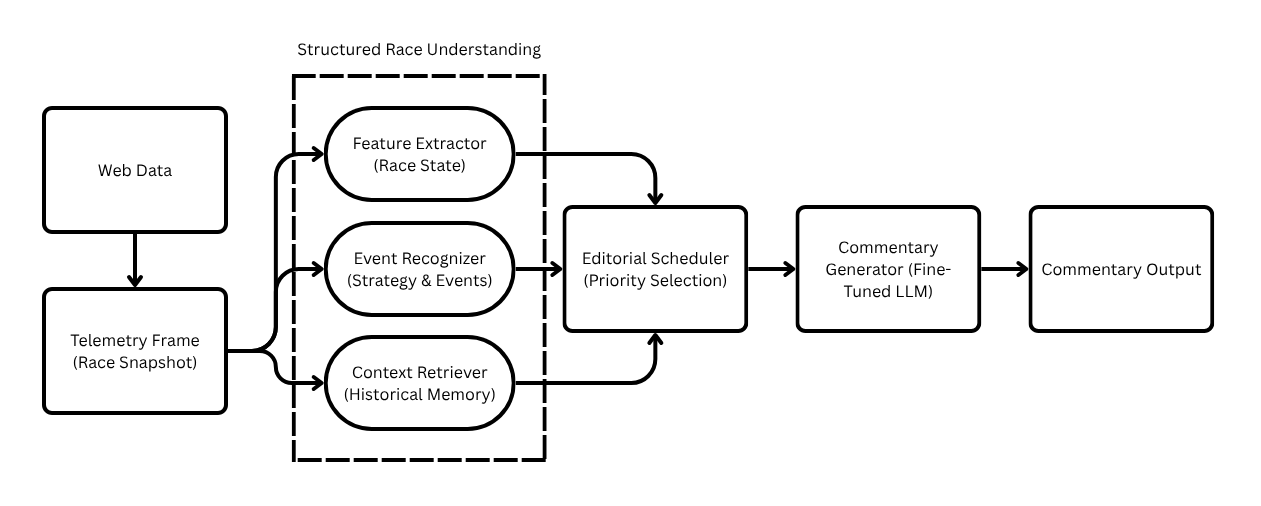
\includegraphics[width=0.9\linewidth]{images/architecture.png}
    \caption{Proposed telemetry-to-narrative architecture. Structured race-state features, event recognition, and contextual retrieval are combined through an editorial scheduler to generate grounded commentary using a fine-tuned language model.}
    \label{fig:architecture}
\end{figure}

As illustrated in Figure~\ref{fig:architecture}, the system follows a structured pipeline that transforms telemetry data into natural language commentary through feature extraction, event recognition, prioritization, and generation.

\subsection{Telemetry Representation}

The input to the system consists of historical Formula 1 telemetry data obtained from FastF1. The data is organized into discrete telemetry frames, where each frame represents a timestamped snapshot of the race.

Each telemetry frame contains per-driver state, including position, lap number, gap to car ahead, tire compound, tire age, and DRS status, as well as global race information such as flag conditions and race control events. These frames serve as the fundamental unit of reasoning and are processed sequentially to simulate a live race environment.

To ensure reproducibility and consistent temporal ordering, telemetry data is processed through a lightweight replay mechanism that emits frames in strict timestamp order.

\subsection{Feature Extraction}

Raw telemetry values are transformed into a structured race-state representation through a feature extraction module. This module computes interpretable features that capture the current dynamics of the race.

The extracted features include gap to car ahead and behind, relative pace differences, tire degradation indicators, DRS availability, pit window relevance, and race control signals. This step defines a structured representation of the race state that enables downstream reasoning over meaningful signals rather than raw numerical inputs.

\subsection{Event and Strategy Recognition}

On top of the extracted features, the system identifies higher-level semantic events using rule-based and heuristic logic. This step converts numerical signals into interpretable race situations.

Detected events include overtake opportunities, pit strategy scenarios such as undercut or overcut potential, tire degradation phases, safety car or yellow flag conditions, and active battles between drivers. This abstraction enables the system to focus on strategic insight rather than direct observation of telemetry values. This approach is consistent with prior work in automated sports commentary, which emphasizes structured event understanding before language generation \cite{AutoBaseComm,AutoBaskComm}.

\subsection{Editorial Scheduling}

Since multiple candidate events may occur simultaneously, the system employs an editorial scheduling mechanism to determine which event should be narrated.

Each candidate event is assigned a priority score based on contextual importance, urgency, race phase, and relevance to ongoing storylines. High-priority events such as lead battles or safety-critical situations are favored over lower-impact developments.

Only the highest-priority event is selected for commentary generation at each time step, while lower-priority events are delayed or suppressed. In addition, a lightweight narrative control mechanism reduces repetition and ensures progression of commentary over time.

\subsection{Context Retrieval}

To enhance commentary with contextual information, the system includes an optional retrieval component based on a local vector database.

When triggered, the system retrieves relevant historical or strategic context, such as prior battles between drivers or recent race developments. Retrieval is gated and only applied to high-priority events in order to maintain low latency and avoid unnecessary overhead.

\subsection{Commentary Generation Model}

The final commentary is generated using a fine tuned language model. We employ the Qwen2.5-7B base model adapted through supervised fine tuning with Low-Rank Adaptation (LoRA) for efficient parameter adaptation.

The fine tuning process follows the supervised fine tuning paradigm, where the model is trained on paired input output examples consisting of structured race state representations and corresponding professional style commentary. During training, the model learns to map structured telemetry derived features and event descriptors to coherent natural language outputs by minimizing the cross entropy loss between predicted and reference tokens. This approach enables the model to align its generation behavior with domain specific linguistic patterns and commentary style \cite{SFT}.

The model takes as input the structured race state representation, the recognized event type, and optional retrieved context. It produces short form commentary describing the current race situation.

The model is optimized to generate commentary that is concise, contextually relevant, and strategically informative, while remaining suitable for real time or near real time usage on consumer hardware. The fine tuning approach follows standard practices for adapting language models to domain specific tasks \cite{SFT}.

A lightweight grounding mechanism is applied during generation to ensure that produced statements remain consistent with the underlying race state and derived features.

\subsection{Dataset Construction}

The training dataset is constructed by aligning telemetry data with professional race commentary. Historical telemetry sequences are segmented into event-centered windows, which are then paired with corresponding commentary transcripts.

Each training example consists of a structured input containing observed facts and derived features, and a target output consisting of the corresponding commentary. This process enables supervised learning of the mapping from telemetry to natural language. The dataset construction strategy is inspired by prior work on sports commentary datasets \cite{AutoBaskData}.

\subsection{System Implementation}

The system is implemented as a lightweight local pipeline to ensure reproducibility and accessibility. Key implementation choices include replay-based telemetry processing, in-memory state tracking, and quantized model inference using local frameworks.

To support evaluation and analysis, the system maintains structured logging of telemetry inputs, generated outputs, and latency measurements. These logs enable reproducibility, debugging, and quantitative comparison across different model configurations.